\documentclass{standalone}
\usepackage{tikz}
\usetikzlibrary{calc} % 坐标计算库
\usetikzlibrary{patterns} % 阴影填充库
\usepackage{pgfplots} % 绘图库
\usepgfplotslibrary{fillbetween} % 区域阴影
\pgfplotsset{compat=1.18} % 设置 pgfplots 版本
\usetikzlibrary{patterns.meta} % 图案库

\begin{document}

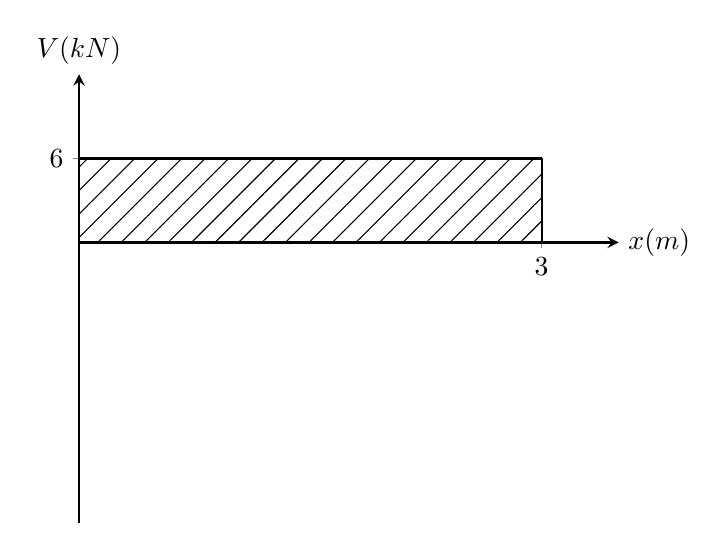
\begin{tikzpicture}
    % Shear Diagram
    % y = 6, 0 <= x <=3
    \begin{axis}[
            axis lines=middle, % 学校式坐标轴
            axis line style={thick},
            xlabel={$x(m)$},
            xlabel style={right},
            ylabel={$V(kN)$},
            ylabel style={above},
            xtick={3},
            ytick={6},
            xmin=0, xmax=3.5,
            ymin=-20, ymax=12,
            domain=0:3,
        ]
        % 定义函数和x轴
        \addplot[name path=A, domain=0:3, thick] {6};
        \addplot[name path=B, domain=0:3] {0};
        % 填充两者之间的区域
        \addplot[
            pattern={Lines[angle=45, distance=6pt]},
        ] fill between [of=A and B];
        % 添加右端分界线
        \draw[thick] (axis cs:3,0) -- (axis cs:3,6);
    \end{axis}

\end{tikzpicture}

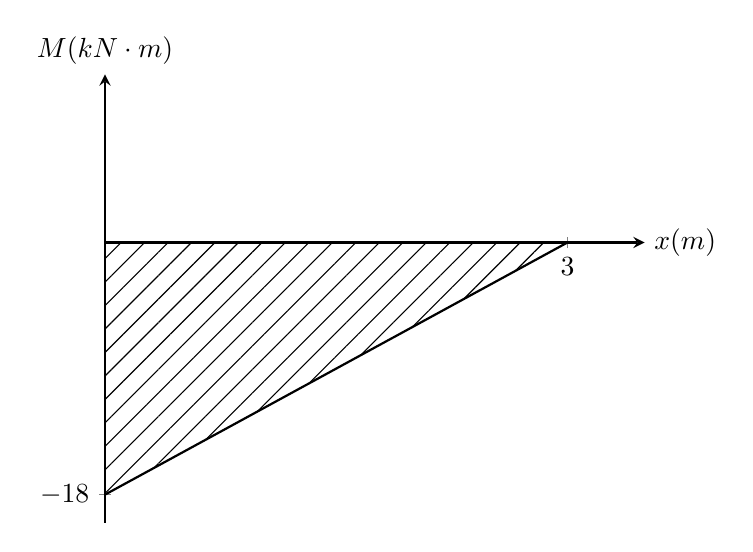
\begin{tikzpicture}
    % Moment Diagram
    % y = 6x - 18, 0 <= x <=3
    \begin{axis}[
            axis lines=middle, % 学校式坐标轴
            axis line style={thick},
            xlabel={$x(m)$},
            xlabel style={right},
            ylabel={$M(kN \cdot m)$},
            ylabel style={above},
            xtick={3},
            ytick={-18},
            xmin=0, xmax=3.5,
            ymin=-20, ymax=12,
            domain=0:3,
        ]
        % 定义函数和x轴
        \addplot[name path=A, domain=0:3, thick] {6*x - 18};
        \addplot[name path=B, domain=0:3] {0};
        % 填充两者之间的区域
        \addplot[
            pattern={Lines[angle=45, distance=6pt]},
        ] fill between [of=A and B];
    \end{axis}

\end{tikzpicture}

\end{document}